\section*{Exercise 4}
\subsection*{rep-24}
The full command we used for retrieving the \textit{csv} file is listed in figure \ref{fig:bash-flowrec}.
\begin{figure}[H]
\begin{lstlisting}[language=bash]
rwcut --num-recs=200000 --delimited=',' --fields=sIP,dIP,sPort,dPort,protocol,flags,ttl,bytes team16.flowrecord.rw > team16_flowrecord.csv
\end{lstlisting}
\caption{ Bash command for retrieving the flow record csv file }
\label{fig:bash-flowrec}
\end{figure}
\subsection*{rep-25}
\begin{table}[H]
\center
\begin{tabular}{lr}
\toprule
port & count \\
\midrule
80 & 31022 \\
0 & 7357 \\
29001 & 1890 \\ 
\bottomrule
\end{tabular}
\caption{ The three most frequent source ports }
\label{tab:most-frequent-source-ports}
\end{table}

\begin{table}[H]
\center
\begin{tabular}{lr}
\toprule
port & count \\
\midrule
445 & 79793 \\
10320 & 32014 \\
3389 & 7834 \\
\bottomrule
\end{tabular}
\caption{ The three most frequent destination ports }
\label{tab:most-frequent-destination-ports}
\end{table}

\begin{table}[H]
\center
\begin{tabular}{lr}
\toprule
protocol & count \\
\midrule
6 (TCP) & 145833 \\ 
17 (UDP) & 46924 \\
1 (ICMP) & 7169 \\
41 (IPv6) & 73 \\
47 (GRE) & 1 \\
\bottomrule
\end{tabular}
\caption{ Frequency of protocols }
\label{tab:all-protocols}
\end{table}

\subsection*{rep-26}
\textbf{TODO}
\subsection*{rep-27}
\textbf{TODO}
\begin{figure}[H]
\center
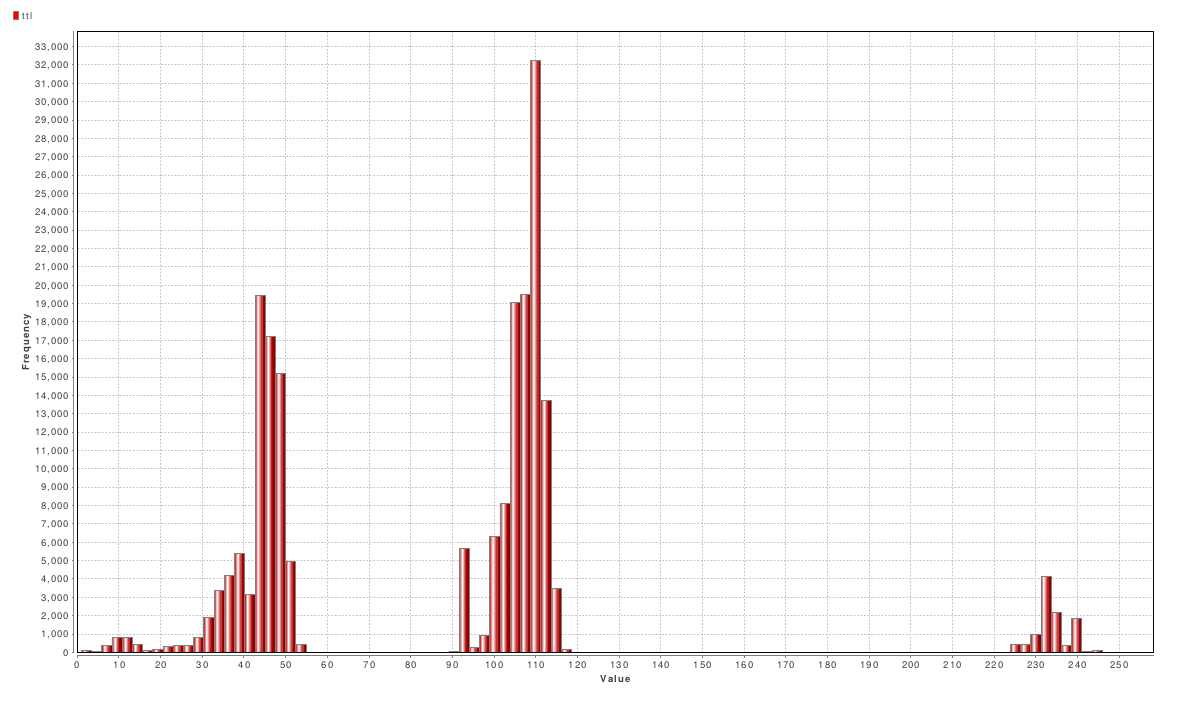
\includegraphics[width=1\textwidth]{./chapters/plots/rep-27-ttl}\\
\caption{TTL distribution of packets}
\label{fig:ttl-distribution}
\end{figure}
\subsection*{rep-28}
The most recurring IP source address is \textbf{85.167.14.252}.
It is easy to find (e.g. by looking at the bytes histogram (figure \ref{fig:bytes-histo}) out that all packets this host sent were of the same size. In addition this host accessed a wide range of IP addresses and a wide range of Ports, therefore it is possible, that this host performed a vertical and horizontal scanning.

\begin{figure}[H]
\center
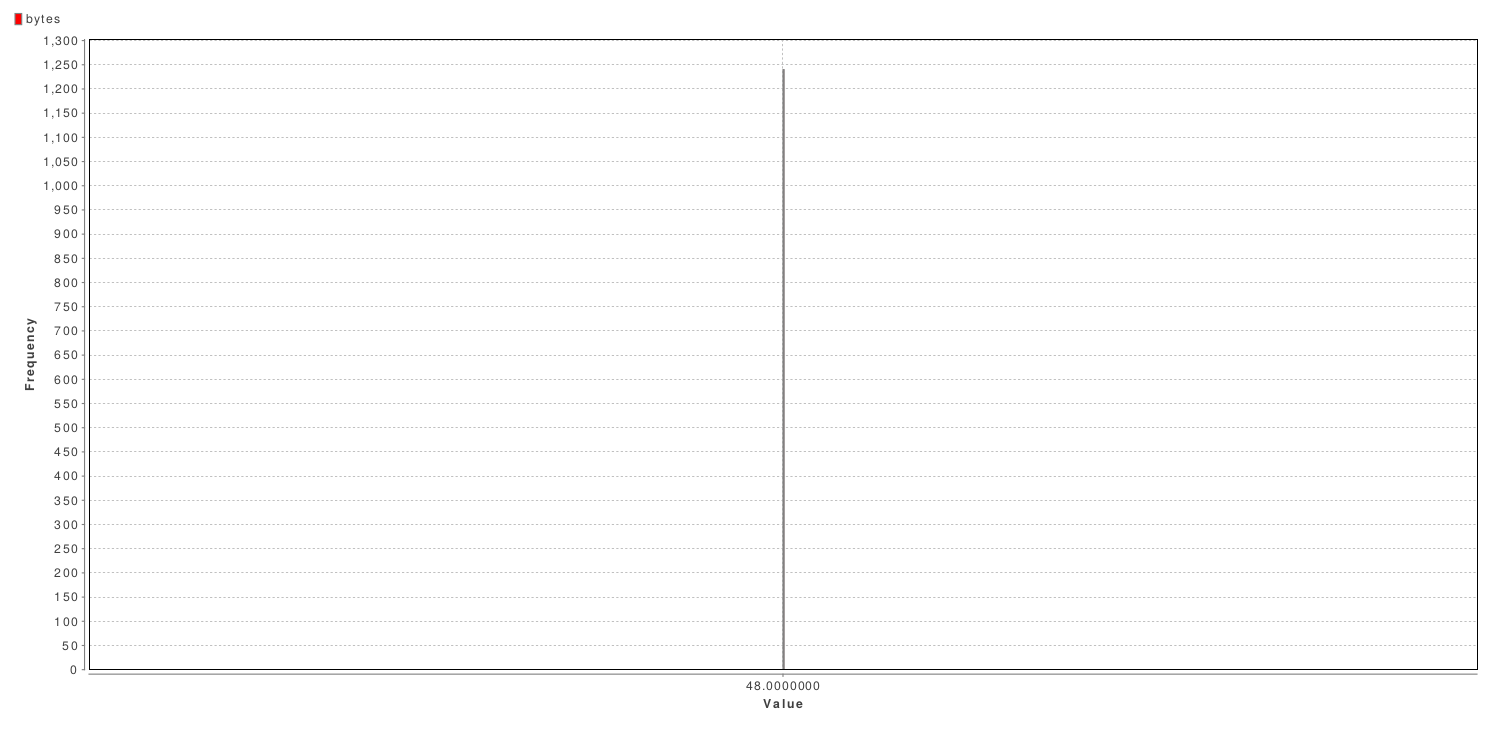
\includegraphics[width=.9\textwidth]{./chapters/plots/rep-28-bytes-histo}\\
\caption{bytes histogramm of all packets sent by 88.167.14.252}
\label{fig:bytes-histo}
\end{figure}

\subsection*{rep-29}
The source IP address, that connected to highest number of destination Ports is again the source IP address \textbf{85.167.14.252}. \\

\textbf{TODO:} explain behavior

\subsection*{rep-30}
The port, that is getting the most connections from different IP sources is the port 445. It is getting IP connections from 79793 different IP sources. It receives the biggest amount of packets from the source IP \textbf{190.253.254.250} (1240 packets). \\

\textbf{TODO: } more detailed discription of the behavior.